\HeaderQuote{But it's no use going back to yesterday, because I was a different person then.}{Alice}

\chapter{Peer-reviewed conference papers}\label{app:confpapers} \todo[color=green!40]{\cref{app:confpapers} Unfinished}

\section[LION5]{Supervised Learning Linear Priority Dispatch Rules for Job-Shop Scheduling}\label{app:lion5}
Supervised Learning Linear Priority Dispatch Rules for Job-Shop Scheduling was 
submitted by \citeauthor{InRu11a} to the 5th International Conference on 
\emph{Learning and Intelligent OptimizatioN Conference} (LION 5), January 
17-21, 2011, Rome, Italy. 
The paper was been accepted as long paper (original novel and unpublished work) 
for presentation at the conference and inclusion in the proceedings. 

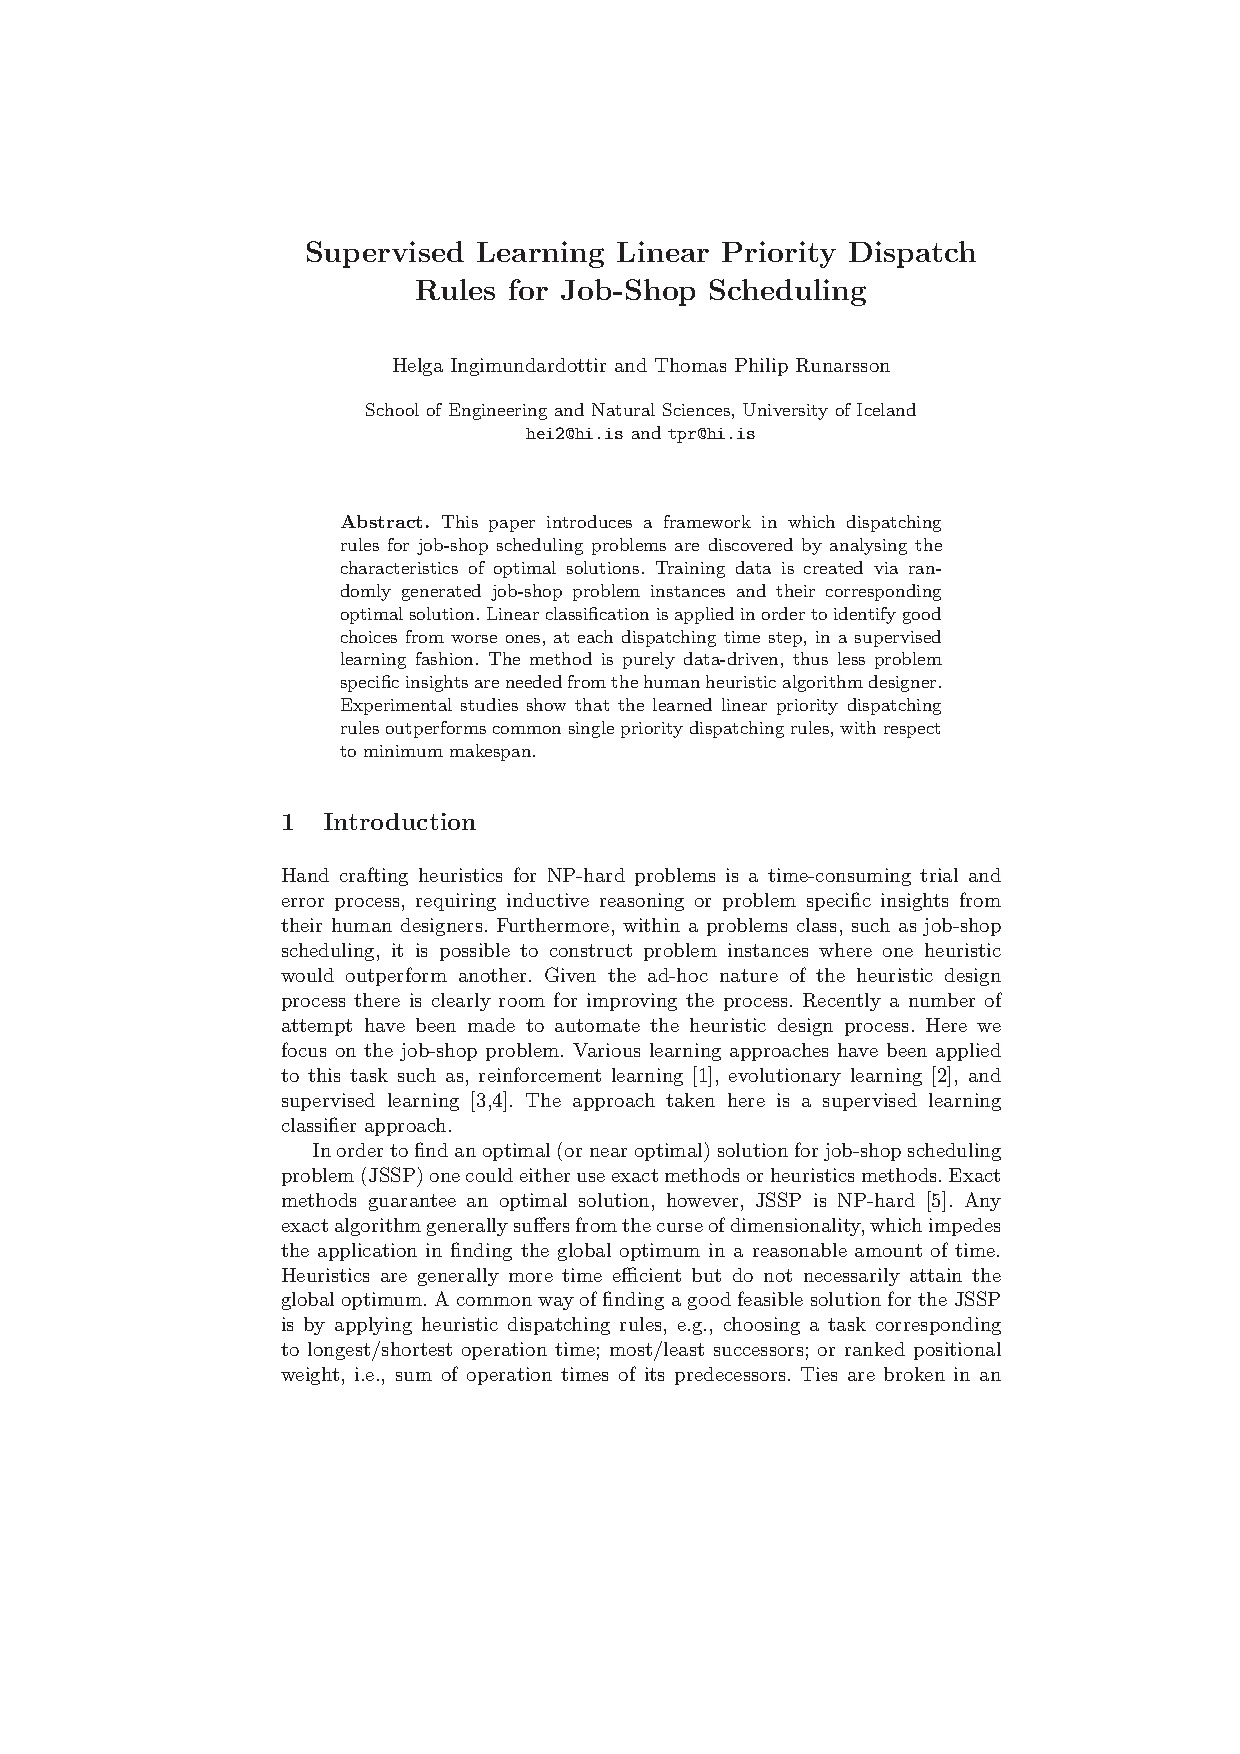
\includepdf[pages=1-15,pagecommand={\thispagestyle{fancy}}]{papers/lion5_linearJSP.pdf}

\section[ISDA11]{Sampling Strategies in Ordinal Regression for Surrogate Assisted Evolutionary Optimization}\label{app:isda2011}
Sampling Strategies in Ordinal Regression for Surrogate Assisted Evolutionary 
Optimization was submitted by \citeauthor{InRu11b} to the 11th International 
Conference on \emph{Intelligent Systems Design and Applications} (ISDA 11), 
November 22-24, 2011, Córdoba, Spain. 
The paper was accepted for presentation at the conference and for publication 
in the conference proceedings published by IEEE.

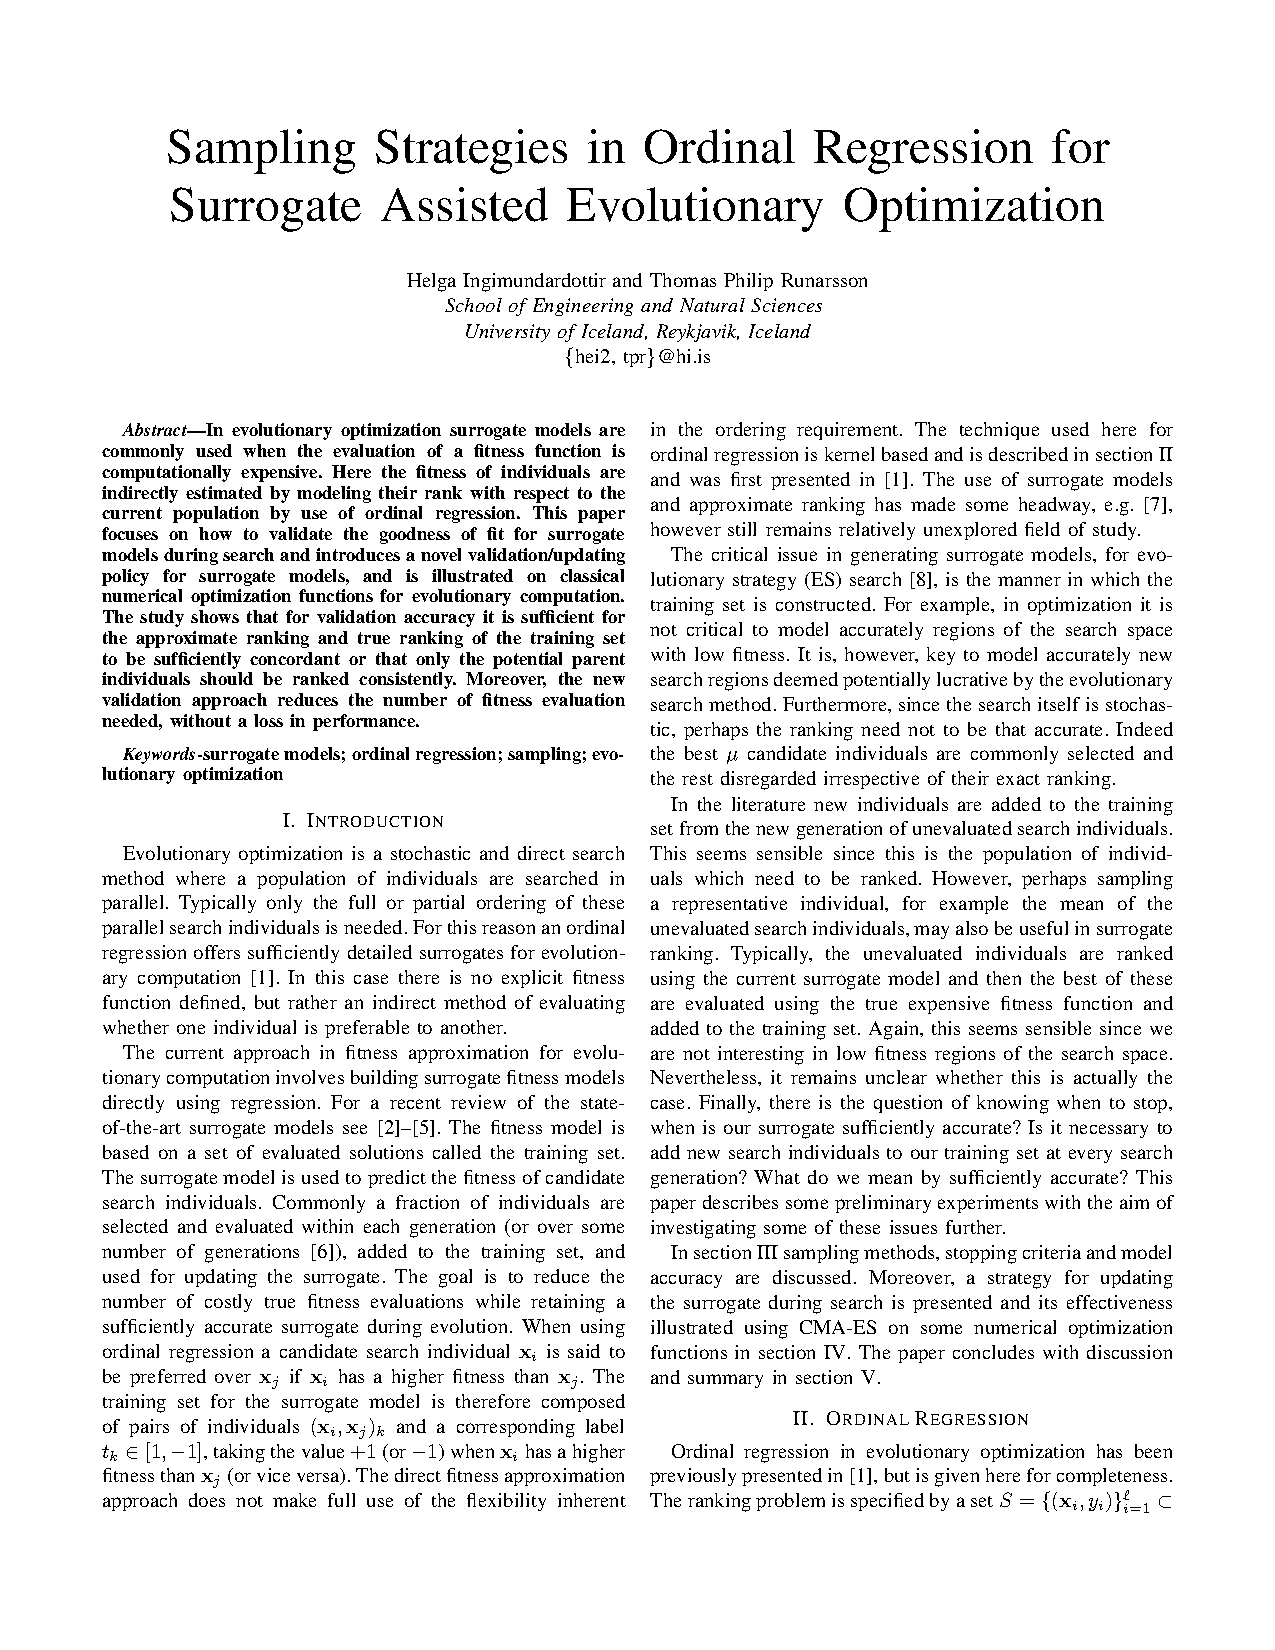
\includepdf[pages=1-6,pagecommand={\thispagestyle{fancy}}]{papers/isda2011.pdf}% ath. ekki blaðsíðutal með á IEEE double-column formattinu. Mögulega hægt ef það væri hægt að scale-a síðurnar betur niður. 

\section[LION6]{Determining the Characteristic of Difficult Job Shop Scheduling Instances for a Heuristic Solution Method}\label{app:lion6}
Determining the Characteristic of Difficult Job Shop Scheduling Instances for a 
Heuristic Solution Method was submitted by \citeauthor{InRu12} to the 6th 
International Conference on \emph{Learning and Intelligent OptimizatioN 
Conference} (LION 6), January 16-20, 2012, Paris, France. 
The paper was been accepted as short paper (an extended abstract of novel work) 
for presentation at the conference and inclusion in the proceedings. 

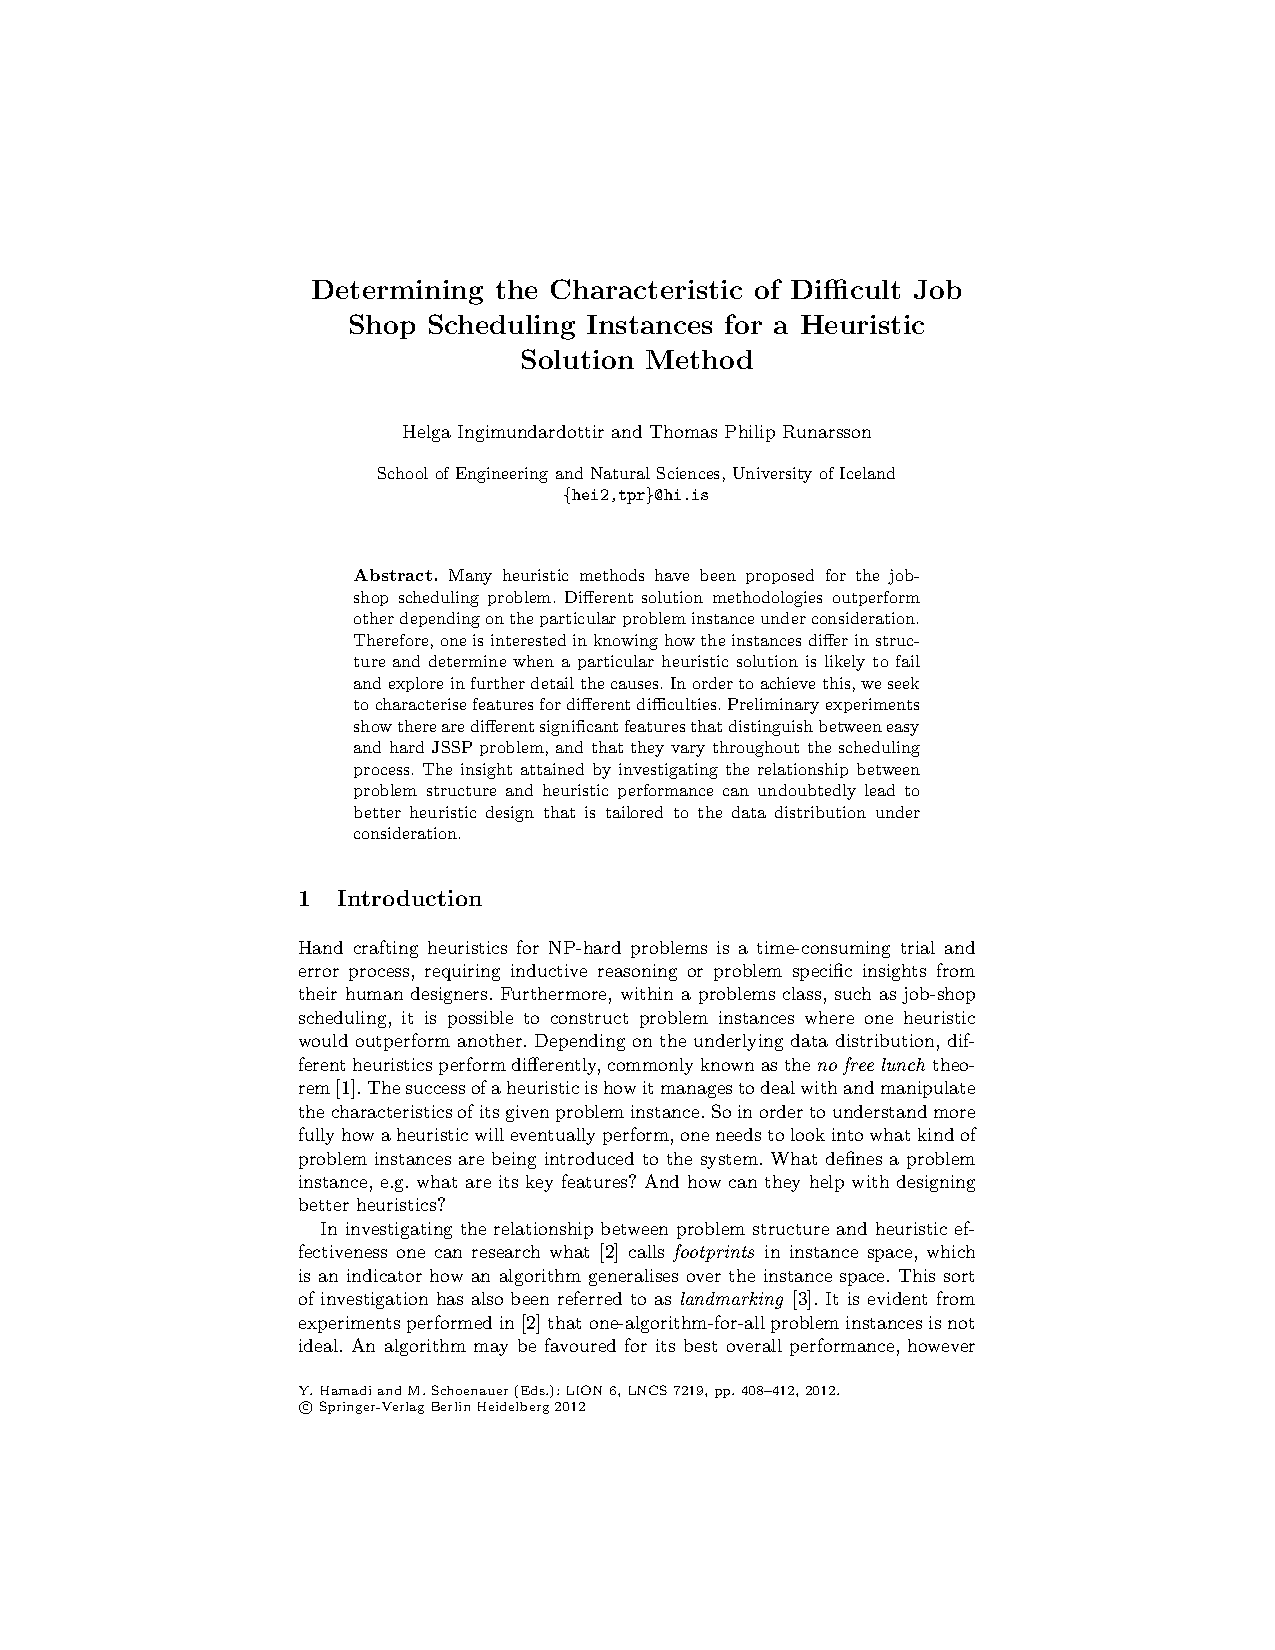
\includepdf[pages=1-5,pagecommand={\thispagestyle{fancy}}]{papers/lion6_easyhardJSSP.pdf}

\section[ECTA6]{Evolutionary Learning of Weighted Linear Composite Dispatching 
Rules for Scheduling}\label{app:ecta6}
Evolutionary Learning of Weighted Linear Composite Dispatching Rules for 
Scheduling was submitted by \citeauthor{InRu14} to the 6th International 
Conference on \emph{Evolutionary Computation Theory and Applications} (ECTA 6), 
October 22-24, 2014, Rome, Italy. 
The paper was been accepted as long paper (original novel and unpublished work) 
for presentation at the conference and inclusion in the proceedings. 

\includepdf[pages=1-9,pagecommand={\thispagestyle{fancy}},noautoscale,scale=0.8]{papers/ecta6_cmaes.pdf}

\section[LION9]{Generating Training Data for Learning Linear Composite 
Dispatching Rules for Scheduling}\label{app:lion9}
Generating Training Data for Learning Linear Composite Dispatching Rules for 
Scheduling was submitted by \citeauthor{InRu15a} to the 9th International 
Conference on \emph{Learning and Intelligent OptimizatioN Conference} (LION 9), 
January 12-16, 2015, Lille, France. 
The paper was been accepted as long paper (original novel and unpublished work) 
for presentation at the conference and inclusion in the proceedings. 
Moreover, the paper was nominated the \emph{Best Paper Award}.

\includepdf[pages=1-14,pagecommand={\thispagestyle{fancy}},noautoscale,scale=0.8]{papers/lion9_gendata.pdf}
